\section{Introducción}
\sangria{} En este trabajo práctico se analizaron diodos rectificadores y zener mediante simulaciones con LTspice y mediciones en laboratorio. Se evaluó su comportamiento en polarización directa e inversa, identificando parámetros clave como la tensión umbral y la zona de ruptura.

\sangria{} Se compararon diodos de silicio (1N4007) y germanio (1N60), utilizando herramientas como Python para graficar curvas I–V y contrastar con los datos experimentales. También se estudiaron aplicaciones prácticas, como circuitos recortadores con diodos zener, integrando conceptos fundamentales para el análisis y diseño de circuitos electrónicos.

\section{Preparación de las prácticas}
\sangria{} Temperatura ambiente del laboratorio al momento de hacer las actividades fue de $25^o$ celsius.
\imagen[Temperatura del laboratorio en ºC]{6cm}{./imagenes/temperaturaAmbiente.jpg}
\sangria{} A continuación se hará mención de los instrumentos de medición utilizados.
\imagen[Instrumentos de medición]{6cm}{./imagenes/instrumentosDeMedición.jpg}
1) \underline{Multímetro}
\begin{itemize}
    \item \textbf{Fabricante:} Pro'sKit
    \item \textbf{Modelo:} MT-1706 CAT 1000V
    \item \textbf{Serie:} MT-17XX
\end{itemize}
\begin{center}
    \begin{tabular}{| p{1cm}  p{1cm}  |}
        \hline
        \multicolumn{2}{|c|}{\textbf{Información de mediciones}} \\
        \hline
        \multicolumn{1}{|m{4cm}}{\centering\textbf{Tensión CC} \\ 60V - Res: 10mV} &
        \multicolumn{1}{|m{3cm}|}{\centering$\pm 0,5\%$ \\+ $3$ dig.} \\
        \hline
        \multicolumn{1}{|m{4cm}}{\centering\textbf{Temperatura $[^oC]$} \\ -20 a 1000$^oC$ - Res: $1^oC$} &
        \multicolumn{1}{|m{3cm}|}{\centering$\pm1,0\% lectura$ \\+ $3$ dig.} \\
        \hline
        \multicolumn{1}{|m{3cm}}{\centering\textbf{Resistencia} \\ $60k\Omega$ - Res: $10\Omega$} &
        \multicolumn{1}{|m{3cm}|}{\centering$\pm 0,8\%$ lectura \\+ $3$ dig.} \\
        \hline
    \end{tabular}
\end{center}

2) \underline{Osciloscopio - multímetro - generador de señales}
\begin{itemize}
    \item \textbf{Fabricante:} FNIRSI
    \item \textbf{Modelo:} 2C23T
    \item \textbf{Serie:} ---
\end{itemize}
\begin{center}
    \begin{tabular}{| p{1cm}  p{1cm}  |}
        \hline
        \multicolumn{2}{|c|}{\textbf{Información de mediciones}} \\
        \hline
        \multicolumn{1}{|m{4cm}}{\centering\textbf{Corriente CC} \\ auto-rango} &
        \multicolumn{1}{|m{3cm}|}{\centering$9999\mu A \rightarrow 9,999A \pm (1,2\%+3)$} \\
        \hline
    \end{tabular}
\end{center}

3) \underline{Multímetro}
\begin{itemize}
    \item \textbf{Fabricante:} BRYMEN
    \item \textbf{Modelo:} BM857S
    \item \textbf{Serie:} BM850A DMM Series
\end{itemize}
\begin{center}
    \begin{tabular}{| p{1cm}  p{1cm}  |}
        \hline
        \multicolumn{2}{|c|}{\textbf{Información de mediciones (modo multímetro)}} \\
        \hline
        \multicolumn{1}{|m{4cm}}{\centering\textbf{Tensión CC} \\ auto-rango} &
        \multicolumn{1}{|m{3cm}|}{$\centering 500mV \rightarrow 50V \pm 0,03\% 2+d$} \\
        \hline
    \end{tabular}
\end{center}

4) \underline{Fuente de tensión continua de la facultad F-44}
\imagen{7cm}{./imagenes/fuenteDeDudosaCalidad.jpg}

\section{Actividad de laboratorio I}
 El objetivo de esta actividad ha sido el de identificar los terminales de los diodos, la comprobación de su correcto funcionamiento y la obtención de la tensión umbral de polarización.
\newpage
 \midTitle{red}{Materiales utilizados}
 \begin{itemize}[noitemsep]
    \item Dos diodos de silicio 1N4007 y otros dos de germanio 1N60. \\
    \begin{center} \diodoSilicio{1N4007} \diodoGermanio{1N60} \end{center}
    \item Multímetro.
    \item Protoboard.
\end{itemize}
\subsection{Identificación de pines y funcionamiento de diodos}
\sangria{} Se colocó el multímetro en modo detección de diodo (mismo que se usa para la continuidad).
\sangria{} Se colocó los diodos en la protoboard, y se procedió a medir los terminales de estos en un sentido y otro.


\begin{center}
    \tikzset{
          hole/.style = {fill = #1, circle, minimum width = 1mm, inner sep = 0mm},
          wire/.style = {draw = #1, line width = 0.2mm},
          label/.style = {rotate = 0, black!50!white, font=\sffamily, anchor = center}
        }
        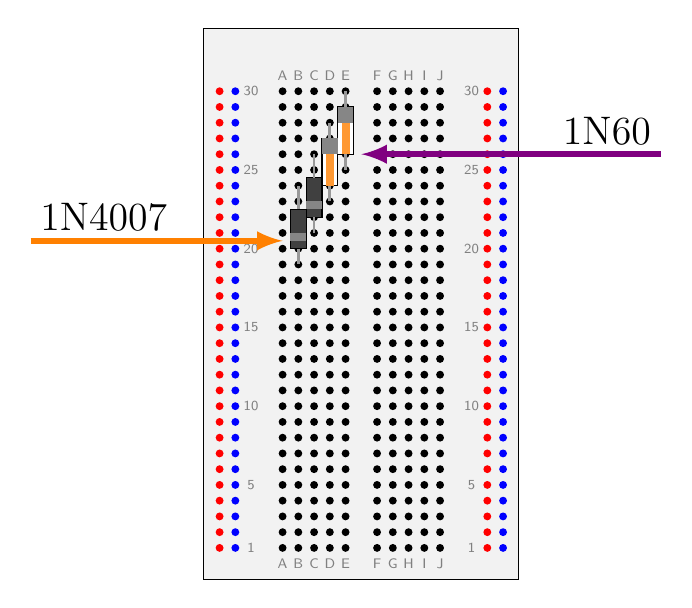
\begin{tikzpicture}[x=2mm,y=2mm]
          \draw[fill=black!05!white] (-4,-1) rectangle (16,34);
 
          \foreach \yi in {1,...,30}{
            \node[hole=red]  at (-3,\yi){};
            \node[hole=blue] at (-2,\yi){};
            \node[hole=red]  at (14,\yi){};
            \node[hole=blue] at (15,\yi){};

            \foreach \xs in {0,6}{
                \foreach \xi in {1,2,3,4,5}{
                    \node[hole=black] at (\xi+\xs,\yi){};
                }
            }
        }

        \foreach \m/\xi in {A/1,B/2,C/3,D/4,E/5,F/7,G/8,H/9,I/10,J/11}{
            \node[label=0] at (\xi, 0) {\tiny\m};
            \node[label=0] at (\xi,31) {\tiny\m};
        }

        \foreach \n/\yi in {1,5,10,15,20,25,30}{
            \node[label=0] at (-1,\yi) {\tiny\n};
            \node[label=0] at (13,\yi) {\tiny\n};
        }  
        \filldraw[fill=white, draw=black] (4.5, 26) rectangle (5.5, 29);
        \fill[fill=orange!80] (4.75, 28) rectangle (5.25, 26);
        \draw[line width=1pt, draw=gray!80] (5, 29) -- (5, 30);
        \draw[line width=1pt, draw=gray!80] (5, 26) -- (5, 25);
        \fill[fill=gray!95] (4.5, 28) rectangle (5.5, 29);

        \filldraw[fill=white, draw=black] (3.5, 24) rectangle (4.5, 27);
        \fill[fill=orange!80] (3.75, 27) rectangle (4.25, 24);
        \draw[line width=1pt, draw=gray!80] (4, 27) -- (4, 28);
        \draw[line width=1pt, draw=gray!80] (4, 24) -- (4, 23);
        \fill[fill=gray!95] (3.5, 26) rectangle (4.5, 27);

        \filldraw[fill=black!75, draw=black] (2.5, 22) rectangle (3.5, 24.5);
        \draw[line width=1pt, draw=gray!80] (3, 24.5) -- (3, 26);
        \draw[line width=1pt, draw=gray!80] (3, 22) -- (3, 21);
        \fill[fill=gray!95] (2.5, 22.5) rectangle (3.5, 23);

        \filldraw[fill=black!75, draw=black] (1.5, 20) rectangle (2.5, 22.5);
        \draw[line width=1pt, draw=gray!80] (2, 22.5) -- (2, 24);
        \draw[line width=1pt, draw=gray!80] (2, 20) -- (2, 19);
        \fill[fill=gray!95] (1.5, 20.5) rectangle (2.5, 21);

        \draw[-latex, very thick, orange, line width=0.75mm] (-15, 20.5) -- (-9, 20.5) -- (1, 20.5);
        \node[anchor=west] at (-15, 22) {\Large 1N4007};

        \draw[-latex, very thick, violet, line width=0.75mm] (25,26) -- (6,26);
        \node[anchor=east] at (25,27.5) {\Large 1N60};

    \end{tikzpicture}
\end{center}

\imagen[Disposición de diodos]{7cm}{./imagenes/disposicionDeDiodos.jpg}

\subsubsection{Valores con el diodo 1N60}
\imagen[Medición en directa]{7cm}{./imagenes/medicionDirecta1N60.jpg}
\imagen[Valores del multímetro en p. directa]{7cm}{./imagenes/medicionDirecta1N60Multimetro.jpg}
\imagen[Medición en inversa]{7cm}{./imagenes/medicionInversa1N60.jpg}
\imagen[Valores del multímetro en p. inversa]{7cm}{./imagenes/medicionInversa1N60Multimetro.jpg}

\begin{center}
\begin{table}[]
    \begin{tabular}{|p{2cm}|p{0.8cm}p{0.9cm}|p{0.8cm}p{0.9cm}|}
\hline
\cellcolor[HTML]{FFFC9E}                                                                                                              & \multicolumn{2}{c|}{\cellcolor[HTML]{FFFFC7}\textbf{1N60}} & \multicolumn{2}{c|}{\cellcolor[HTML]{FF9390}\textbf{1N4007}} \\ \cline{2-5} 
\multirow{-2}{*}{\cellcolor[HTML]{FFFC9E}\textbf{\begin{tabular}[c]{@{}c@{}}Sentido de las \\ puntas del \\ multímetro\end{tabular}}} & \multicolumn{1}{c|}{\textbf{D1}}        & \textbf{D2}        & \multicolumn{1}{c|}{\textbf{D1}}       & \textbf{D2}       \\[12pt] \hline
\begin{tabular}[c]{@{}c@{}}Polarización \\ directa\end{tabular}                                                                       & \multicolumn{1}{c|}{0,373V}             & 0,401V             & \multicolumn{1}{c|}{0,593V}            & 0,614V            \\ \hline
\begin{tabular}[c]{@{}c@{}}Polarización \\ inversa\end{tabular}                                                                       & \multicolumn{1}{c|}{0V}                 & 0V                 & \multicolumn{1}{c|}{0V}                & 0V                \\ \hline
\end{tabular}
\end{table}
\end{center}

\begin{figure}[H]
    \centering
    \begin{subfigure}[b]{0.45\linewidth}
        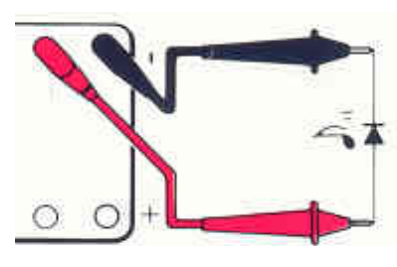
\includegraphics[width=3.5cm]{./imagenes/polarizacionDirecta.png}
        \caption{Polarización Directa}
    \end{subfigure}
    \hfill
    \begin{subfigure}[b]{0.45\linewidth}
        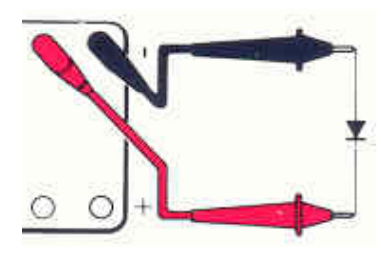
\includegraphics[width=3.5cm]{./imagenes/polarizacionInversa.png}
        \caption{Polarización Inversa}
    \end{subfigure}
    \caption{Modos de polarización del diodo}
    \label{fig:polarizaciones}
\end{figure}

\subsection{Conclusión de la identificación de pines}
\sangria{} Se identificaron correctamente los terminales de los diodos 1N4007 y 1N60 utilizando el multímetro en modo de prueba de diodos. Se verificó que, al aplicar la polarización directa, los diodos condujeron corriente mostrando una caída de tensión en el rango esperable para cada tecnología: aproximadamente 0,6V para el 1N4007 (silicio) y entre 0,37V y 0,4V para el 1N60 (germanio).

\sangria{} En polarización inversa, ambos diodos bloquearon el paso de corriente, como se esperaba, indicando que no presentaban fallas internas. A partir de estas pruebas simples pero efectivas, se lograron identificar el ánodo y el cátodo en cada diodo, permitiendo su correcta utilización.

